\documentclass{beamer}
\usetheme{default}
%\usetheme{Boadilla}
\usepackage[english]{babel}
\usepackage[T1]{fontenc}
\usepackage[utf8]{inputenc}
\usepackage{times}
\parindent0em

\usepackage{graphicx}
\usepackage{float}
\inputencoding{utf8}
\usepackage{multicol}
\usepackage{vwcol} 
\usepackage{color}
\definecolor{links}{HTML}{2A1B81}
\hypersetup{colorlinks,linkcolor=,urlcolor=links}
\usepackage{listings}

\definecolor{keywords}{RGB}{255,0,90}
\definecolor{comments}{RGB}{0,0,113}
\definecolor{red}{RGB}{160,0,0}
\definecolor{green}{RGB}{0,150,0}
 
\lstset{language=Python, 
        basicstyle=\ttfamily\small, 
        keywordstyle=\color{keywords},
        commentstyle=\color{comments},
        stringstyle=\color{red},
        showstringspaces=false,
        identifierstyle=\color{green},
        procnamekeys={def,class}}


\begin{document}

\title[Group Project]{Simple Course Management System}
\author{Antigravity - Chris Papke, Jimmy Pardey, \\Stefanie Fritz, Thomas Watkin}
\date{\today}

\begin{frame}[plain]
\titlepage
\end{frame}

\begin{frame}[fragile]
\frametitle{Implementation Technology}
\begin{itemize}
	\item Python
	\item Django
	\item Postgres
\end{itemize}
\end{frame}

\begin{frame}[fragile]
\frametitle{Conceptual Data Model}

\begin{figure}
	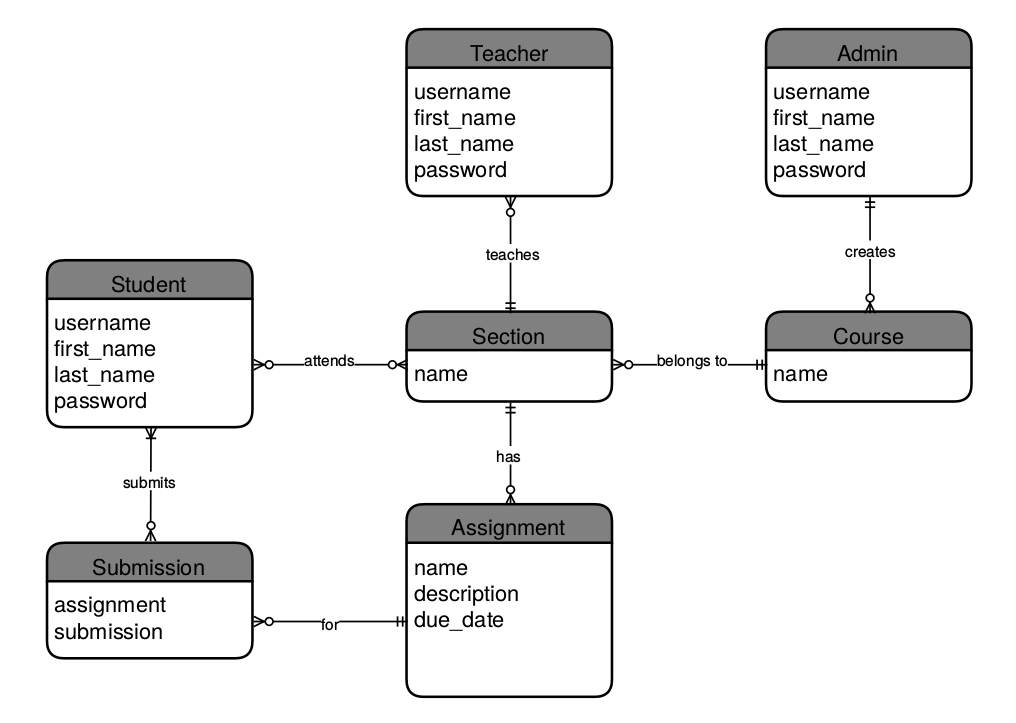
\includegraphics[width=\textwidth]{concept.png}
\end{figure}
\end{frame}


\begin{frame}[fragile]
\frametitle{Model}

\begin{lstlisting}[basicstyle=\small]
class Assignment(models.Model):
    name = models.CharField(max_length=255)
    section = models.ForeignKey('courses.Section', 
        related_name='assignments')
    description = models.TextField()
    due_date = models.DateTimeField()

    def __str__(self):
        return str(self.section) + " - " + self.name
\end{lstlisting}
\end{frame}

\begin{frame}[fragile]
\frametitle{View}

\begin{lstlisting}[basicstyle=\tiny]
@login_required
@get_request_user
def user_profile(request, user):
    sections = []
    assignments = []
    if user.is_teacher():
        sections = Section.objects.filter(teacher=user.id)
        context = {'user': user, 'sections': sections}
    elif user.is_student():
        due_assignments = []
        sections = Section.objects.select_related('course')\
            .prefetch_related('assignments').filter(students=user.id)
        for section in sections:
            assignments.extend(section.assignments.all())
        for assignment in assignments:
            if assignment.due_date > timezone.now():
                due_assignments.append(assignment)
        context = {'user': user, 'sections': sections, 
            'assignments': assignments, 'due_assignments': due_assignments}

    return render(request, 'users/profile.html', context)  
\end{lstlisting}
\end{frame}


\lstset{%
  basicstyle=\ttfamily,
  breaklines=true,
  columns=fullflexible,
  showstringspaces=false,
  language=HTML,
  identifierstyle=\color{magenta!50!black},
  stringstyle=\color{blue}
}


\begin{frame}[fragile]
\frametitle{Template}

\begin{lstlisting}[basicstyle=\tiny]


<h3>Join the Section</h3>
<form action="" method="post">
    
    <input type="submit" value="Join" />
</form>

<h3>Add students to section</h3>
<form action="" method="post">
    
    <label for="student_id">Student</label><br />
    <select name=student_id id=student_id >
    
        <option value={{student.id}}>{{student}}</option>
    
    </select>
    <input type="submit" value="Add student" />
</form>

  
\end{lstlisting}
\end{frame}


\begin{frame}[fragile]
\frametitle{What we learned}

\begin{itemize}
	\item Python \& Django are very powerful
	\item 
\end{itemize}

\end{frame}



\end{document}